% !TeX encoding = UTF-8
% !TeX program = pdflatex
% !TeX spellcheck = en_US

\documentclass{article}

\usepackage[utf8]{inputenc}
%\usepackage{fourier}
%\usepackage{array}
\usepackage{makecell}
\usepackage{graphicx}
\usepackage{todonotes}
\usepackage{subcaption}

\begin{document}

\section{Experiments}

In this section, we report the
experimental result of our implementation
of Algorithm 1 and 2 presented in previous sections,
in the following called \texttt{pac-rdp} and \texttt{pac-rdp-simple},
respectively.
As baseline, we consider vanilla Q-Learning (\texttt{q-learning}),
trained with $\epsilon$-greedy policy with $\epsilon=0.1$
and learning rate $\alpha = 0.1$.
For Algorithm 2, instead of running
\texttt{AdaCT} every episode, we
run it every 500 episodes; This simplifies
the benchmarking, because the workload
for each episode would have been too high, without
much benefits.

In all the experiments,
we run the greddy policy for 50 episodes, with the currently learned model,
every 500 training episodes, and collect
the average reward obtained across the test episodes.
Each experiment is run $8$ times
\todo{In the final version, the number of runs will be increased},
and the plots
show the average reward and the standard deviation
of the optimal policy during the training, as explained above.


\subsection{Rotating MAB}

The configurations for this experiments are reported in
Table~\ref{tab:rotmab-params}.

\begin{table}[!h]
\centering
    \begin{tabular}{|c|c|c|}
 \hline
 Parameter & Description & Value \\ \hline \hline
 $n$ & Number of arms & $2$\\ \hline
 $\gamma$ & Discount factor & $0.99$\\ \hline
 $\epsilon$ & Accuracy & $0.05$\\ \hline
 $\delta$ & Condifidence & $0.05$\\ \hline
 $r$ & Success reward & $1$\\ \hline
 $(p_1, p_2)$ & Success probabilities & $(0.9, 0.2)$\\ \hline
 $N$ & Number of episodes & 50000 \\ \hline
 $M$ & Maximum number of steps per episode & 100 \\ \hline
 $\ell_{\max}$ & Maximum state upperbound for \texttt{pac-rdp} & 10 \\ \hline
 $\hat{D}$ & Upperbound on depth for \texttt{pac-rdp-simple} & 10 \\ \hline
\end{tabular}
\caption{Parameters for Rotating MAB experiment.}
 \label{tab:rotmab-params}
\end{table}

The results are shown in Figure~\ref{fig:rotmab-experiment}.
The last model learned as PDFA is shown in Figure~\ref{fig:rotmab-pdfa}.

\begin{figure}[!h]
 \centering
 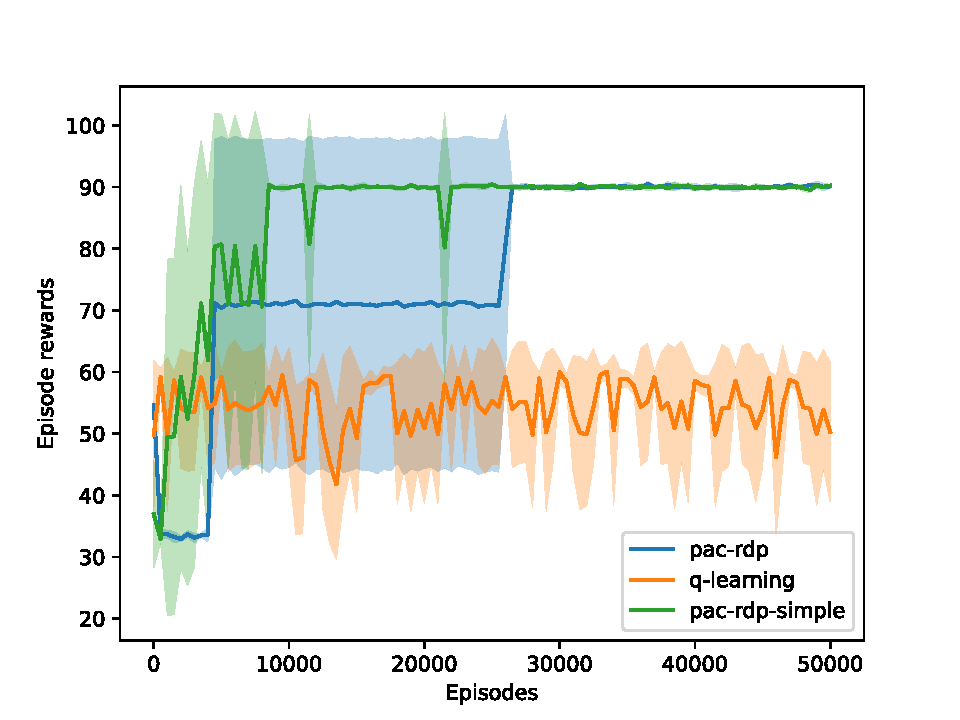
\includegraphics[width=\linewidth]{plot-rotmab.pdf}
 \caption{Average episode rewards of the greedy policy for Rotating MAB. The optimal average reward
 is $M\cdot p_{\max} \cdot r = 0.9$, that is, when the agent always knows the current state of the
 shifts and the most rewarding arm to pull.}
 \label{fig:rotmab-experiment}
\end{figure}%
\begin{figure}[!h]
 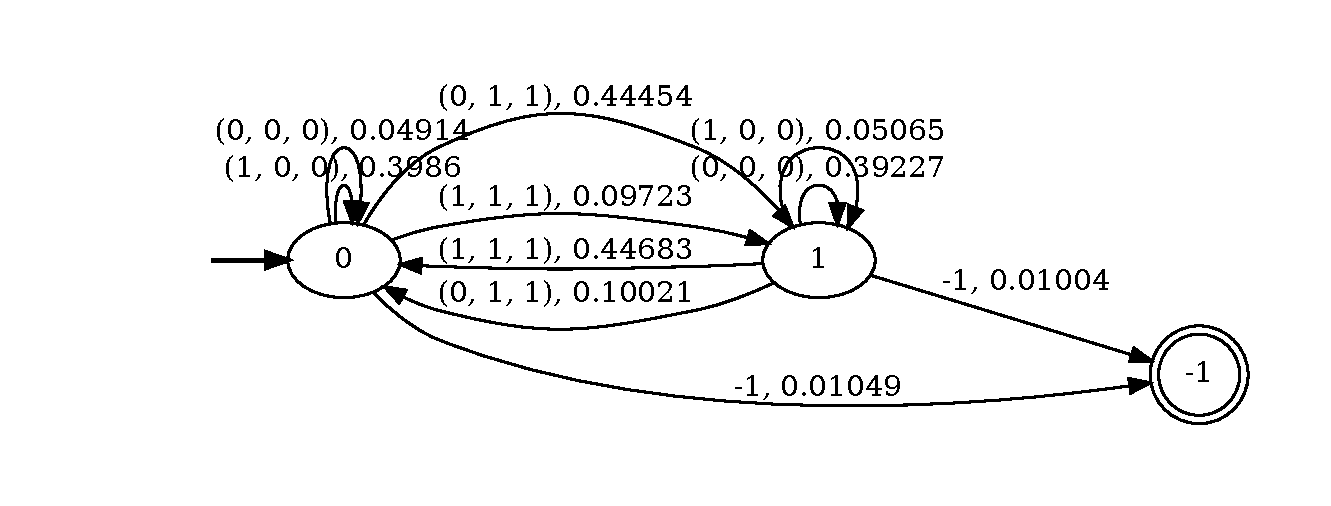
\includegraphics[width=\linewidth]{pdfa-rotmab-02-90-20.pdf}
 \caption{The PDFA for Rotating MAB $(p_1, p_2)$. The
   transition is made only when a reward is observed (i.e. the middle number
 of the triple $(a, r, s)$.)}
 \label{fig:rotmab-pdfa}
\end{figure}

\pagebreak

\subsection{Cheat MAB}

The configurations for this experiments are reported in
Table~\ref{tab:cheatmab-params}.

\begin{table}[!h]
\centering
    \begin{tabular}{|c|c|c|}
 \hline
 Parameter & Description & Value \\ \hline \hline
 $n$ & Number of arms & $2$\\ \hline
 $\gamma$ & Discount factor & $0.99$\\ \hline
 $\epsilon$ & Accuracy & $0.05$\\ \hline
 $\delta$ & Condifidence & $0.05$\\ \hline
 $r$ & Success reward & $1$\\ \hline
 $P$ & Pattern to complete & $[0, 0, 1]$\\ \hline
 $N$ & Number of episodes & 50000 \\ \hline
 $M$ & Maximum number of steps per episode & 100 \\ \hline
 $\ell_{\max}$ & Maximum state upperbound for \texttt{pac-rdp} & 10 \\ \hline
 $\hat{D}$ & Upperbound on depth for \texttt{pac-rdp-simple} & 10 \\ \hline
\end{tabular}
\caption{Parameters for Cheat MAB experiment.}
\label{tab:cheatmab-params}
\end{table}

The results are shown in Figure~\ref{fig:cheatmab-experiment}.
The last model learned as PDFA is shown in Figure~\ref{fig:cheatmab-pdfa}.

\begin{figure}[!h]
 \centering
 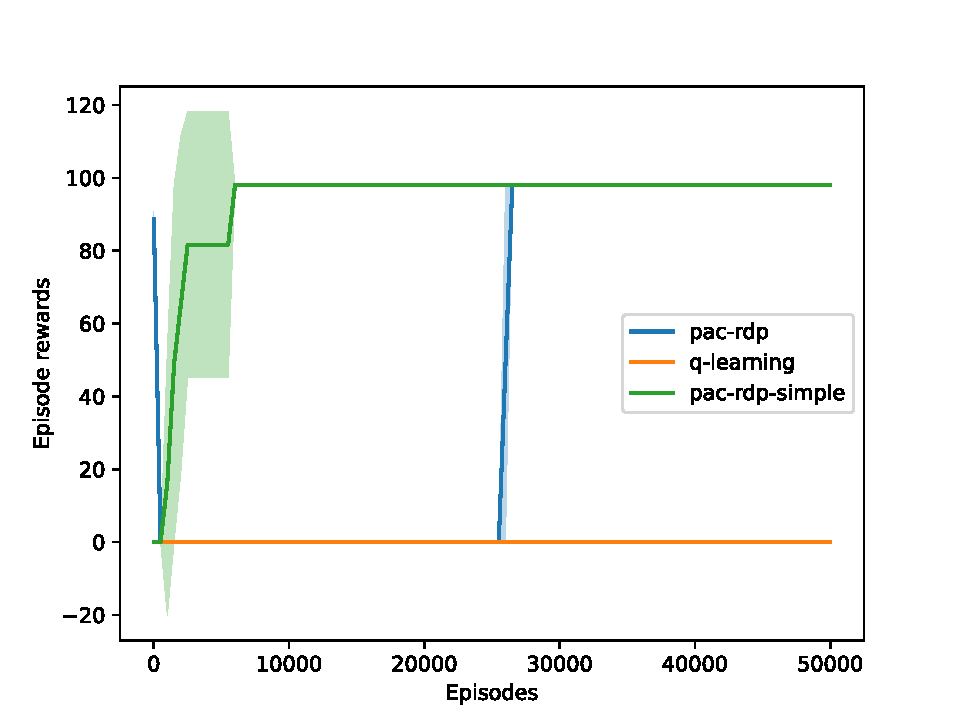
\includegraphics[width=\linewidth]{plot-cheatmab.pdf}
 \caption{Average episode rewards of the greedy policy for Cheat MAB.
 The optimal average reward is $(M - length(P) + 1)\cdot r = 98.0$,
 that is, when the agent completes the pattern as soon as possible.}
 \label{fig:cheatmab-experiment}
\end{figure}%
\begin{figure}[!h]
 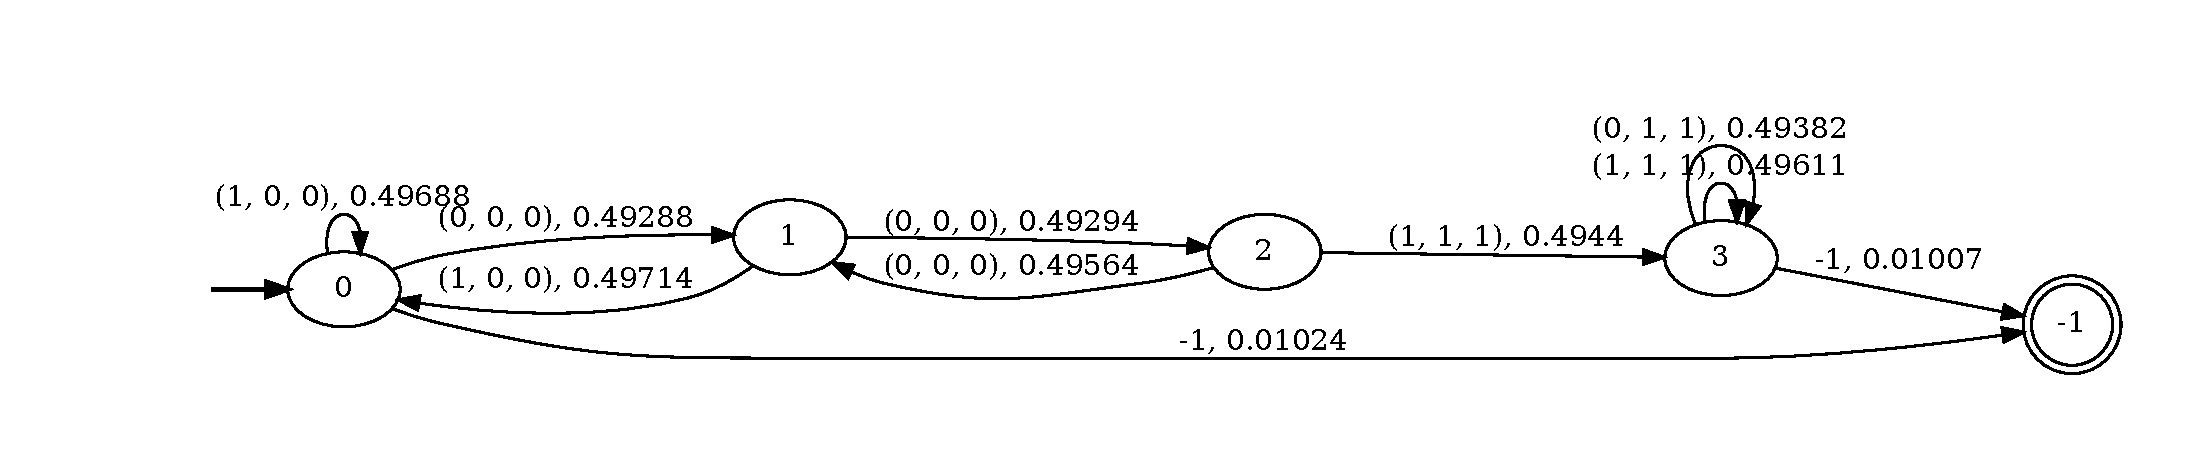
\includegraphics[width=\linewidth]{pdfa-cheatmab-02-001.pdf}
 \caption{The PDFA for Cheat MAB. The
   transition is made only when the first number, corresponding
 to the chosen action, is the right action for the pattern.
 In this case, the pattern is: two times the action $0$, and
 one time the action $1$. After the pattern is completed, reward is always 1,
 regardless of the actual action.}
 \label{fig:cheatmab-pdfa}
\end{figure}

\pagebreak


\subsection{Malfunction MAB}

The configurations for this experiments are reported in
Table~\ref{tab:malfunctionmab-params}.

\begin{table}[!h]
\centering
    \begin{tabular}{|c|c|c|}
 \hline
 Parameter & Description & Value \\ \hline \hline
 $n$ & Number of arms & $2$\\ \hline
 $\gamma$ & Discount factor & $0.99$\\ \hline
 $\epsilon$ & Accuracy & $0.05$\\ \hline
 $\delta$ & Condifidence & $0.05$\\ \hline
 $r$ & Success reward & $1$\\ \hline
 $(p_1, p_2)$ & Success probabilities & $(0.2, 0.8)$\\ \hline
 $k$ & No. times to break an arm & $2$\\ \hline
 $N$ & Number of episodes & $75000$ \\ \hline
 $M$ & Maximum number of steps per episode & 100 \\ \hline
 $\ell_{\max}$ & Maximum state upperbound for \texttt{pac-rdp} & 10 \\ \hline
 $\hat{D}$ & Upperbound on depth for \texttt{pac-rdp-simple} & 10 \\ \hline
\end{tabular}
\caption{Parameters for Malfunction MAB experiment.}
\label{tab:malfunctionmab-params}
\end{table}

The results are shown in Figure~\ref{fig:malfunctionmab-experiment}.
The last model learned as PDFA is shown in Figure~\ref{fig:malfunctionmab-pdfa}.

\begin{figure}[!h]
 \centering
 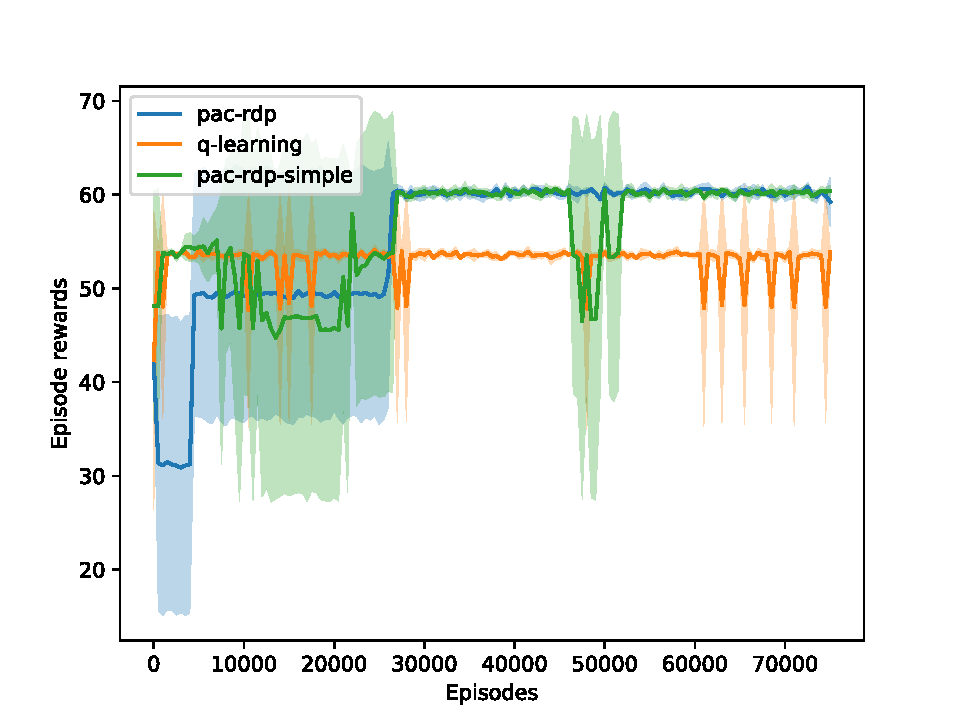
\includegraphics[width=\linewidth]{plot-malfunctionmab.pdf}
 \caption{Average episode rewards of the greedy policy for Malfunction MAB.
 The optimal average reward is the one obtained by
 pulling the best arm when it is working, and the second best arm
 in case the first is not working.
 More precisely, in this case, the optimal average reward is:
 $Mr(p_1(\frac{k}{k+1}) + p_2(\frac{1}{k+1})) = 60.0$, i.e. the weighted
 average between the first best (malfunctioning) arm and the second best
 (working) arm.}
 \label{fig:malfunctionmab-experiment}
\end{figure}%
\begin{figure}[!h]
 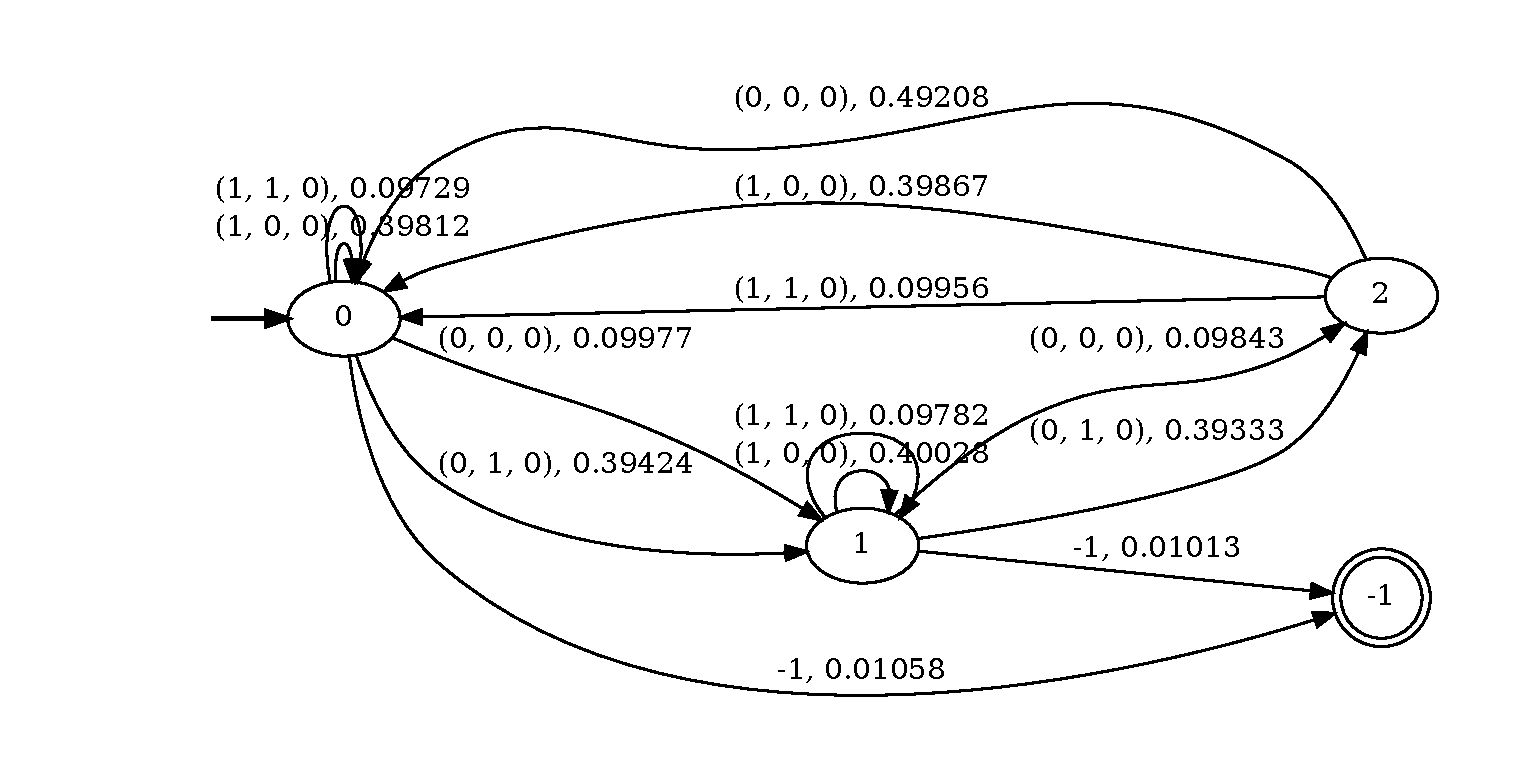
\includegraphics[width=\linewidth]{pdfa-malfunctionmab-02-80-20.pdf}
 \caption{The PDFA for Malfunction MAB. The PDFA reduces
 to a counter up to $k$, which increases only when the first arm is pulled.
 After being in state $k$, whatever is the next action,
 the episode goes to the initial state.}
 \label{fig:malfunctionmab-pdfa}
\end{figure}

\pagebreak


\subsection{Driving Agent}

The configurations for this experiments are reported in
Table~\ref{tab:drivingagent-params}.

\begin{table}[!h]
\centering
    \begin{tabular}{|c|c|c|}
 \hline
 Parameter & Description & Value \\ \hline \hline
 $\gamma$ & Discount factor & $0.99$\\ \hline
 $\epsilon$ & Accuracy & $0.05$\\ \hline
 $\delta$ & Condifidence & $0.05$\\ \hline
 $N$ & Number of episodes & 50000 \\ \hline
 $M$ & Maximum number of steps per episode & 100 \\ \hline
 $\ell_{\max}$ & Maximum state upperbound for \texttt{pac-rdp} & 10 \\ \hline
 $\hat{D}$ & Upperbound on depth for \texttt{pac-rdp-simple} & 10 \\ \hline
\end{tabular}
\caption{Parameters for Driving Agent experiment.}
\label{tab:drivingagent-params}
\end{table}

The results are shown in Figure~\ref{fig:drivingagent-experiment}.
The last model learned as PDFA is shown in Figure~\ref{fig:drivingagent-pdfa}.

\begin{figure}[!h]
 \centering
 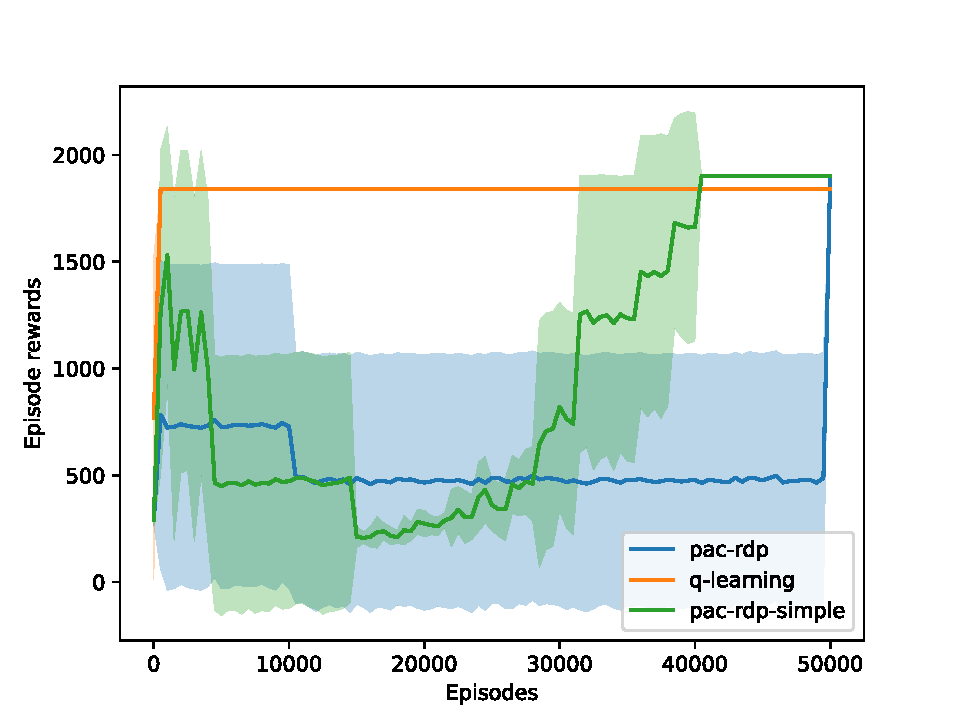
\includegraphics[width=\linewidth]{plot-drivingagent.pdf}
 \caption{Average episode rewards of the greedy policy for Driving Agent.
 The optimal average reward is the one obtained by
 driving slowly when it has been rainy and not sunny since then,
 and driving normally elsewhere. Q-Learning only learns to drive
 slowly when not sunny and normally when sunny; however, this is suboptimal,
 because when cloudy you may drive normally if it has been sunny and not rainy recently.}
 \label{fig:drivingagent-experiment}
\end{figure}%
\begin{figure}[!h]
 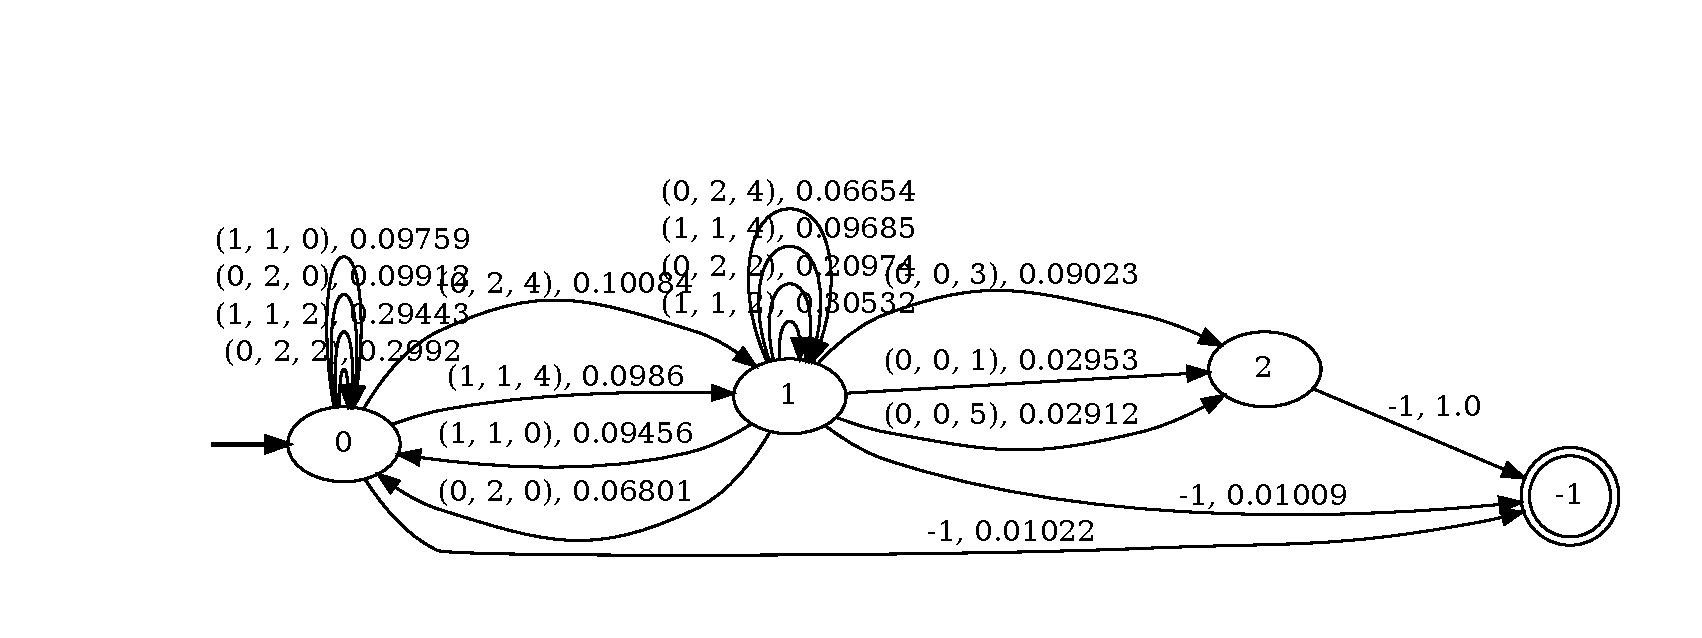
\includegraphics[width=\linewidth]{pdfa-driving_agent.pdf}
 \caption{The PDFA for the Driving Agent environment.
 Action with index $0$ is "driving normally", whereas index $1$ is "driving slowly".
 The indices for the rewards are $0$ for $r=0$, $1$ for $r=18$ and $2$ for $r=20$.
 The indices for the observations $S$ are: even numbers $0$, $2$ and $4$ for, respectively,
 $sunny$, $cloudy$ and $rainy$ with no accident; odd numbers $1$, $3$ and $5$
 in case an accident is happened.
 State $0$ represents the condition when it has not been rainy recently.
 When in state $1$, it means it has been rainy and not sunny.
 State $2$ means an accident is happened.}
 \label{fig:drivingagent-pdfa}
\end{figure}

\end{document}
